% *****************************************************
%
% DESIGN - State the identified requirements and show
% design diagrams with full explanations for product.
%
% *****************************************************
\chapter{Design} \label{chap:design}
This chapter covers the decisions made and the reasoning behind these decisions during the design and planning stage before the implementation phase of this project. It will first cover what was decided what the requirements of the product were going to be, before a high-level discussion and comparison of design methodologies that would be suitable for this project. This chapter will also discuss and compare all the languages, tools and services that could have been chosen to be used for implementation and provide all the plans and diagrams used for planning the project.
\section{Product Requirements}
When thinking about and documenting the requirements of the product, two well-known and popular frameworks are, the user stories framework and the jobs to be done framework. The user stories framework allows requirements to be written from the perspective of a user/persona and the jobs to be done framework allows requirements to be written to set out actions that are executed when a specified event is triggered. From a high level, the statement for the overall requirement for the product is as follows:\\\\
\textbf{``A chatterbot that allows a user to login/signup and converse with the chatterbot. Additionally, the chatterbot will be connected with a database and have a long-term memory mechanism that allows it to remember conversation."}\\\\
The jobs to be done framework was chosen, for writing the requirements as there aren't really multiple user groups and this framework is useful for documenting, at a high level, all the events that could occur and their expected outcomes. Additionally, the requirements were broken down into two categories, functional and non-functional requirements. Functional requirements are those that are concerned with features of the system, such as logging into the app, whilst non-functional requirements are concerned with how well the system should perform, such as system security and ease of use.\\
Listed below are all of the functional and non-functional requirements for the system. Each requirement has a corresponding priority, with Priority 1 being of the highest priority and Priority 4 being the lowest.
\subsection{Functional Requirements} \label{ssection:functional}
% Long list of functional requirements go here...
\begin{enumerate}
	\item When a user visits the chatterbot for the first time, they should be able to signup, so they can interact with the chatterbot. \textbf{Priority 1}
	\item When a user returns to the chatterbot, they should be able to login, so that they can interact with the chatterbot again. \textbf{Priority 1}
	\item When a user logs in, the chatterbot should display all the previous messages in the chat, so that the user can see and refer back to them. \textbf{Priority 1}
	\item When a user is logged in, they should be able to send a message to the chatterbot, so that they can converse with the chatterbot. \textbf{Priority 1}
	\item When the chatterbot receives a message from a user, the chatterbot should send a message back, so the user can receive a response to their user and continue the conversation. \textbf{Priority 1}
	\item When the chatterbot receives a message from a user, the chatterbot should access the past conversations with the user, so that the chatterbot can see if it can refer back to any topics or entities in the current conversation and change the current topic of the conversation accordingly. \textbf{Priority 1}
	\item When the chatterbot responds to a message from the user, both the user's message and the chatterbot's response should be displayed, so the user can see and follow the conversation. \textbf{Priority 1}
	\item When any messages are sent to/from the chatterbot, both the user's message and the chatterbot's response should be stored, so the user can see the past conversation and the chatterbot can access the past conversation. \textbf{Priority 1}
	\item When a user logs in, the chatterbot should send a generic greeting to the user, so that the user feels welcome and it serves as a conversation starter. \textbf{Priority 2}
	\item When a user logs in, the chatterbot should send a personalised greeting, based on the user's sentiment from the last time the user conversed with the chatterbot, so that the chatterbot can gauge the user's current mood. \textbf{Priority 3}
	\item When a user is logged in, the user should have an option to sign out, so that the user can safely exit the program. \textbf{Priority 3}
	\item When a user sends a message, there should be a short delay before the response is displayed, so that the user thinks that they are talking to a human. \textbf{Priority 4}
\end{enumerate}
\subsection{Non-Functional Requirements} \label{ssection:non-functional}
% Short list of non-functional requirements go here...
\begin{enumerate}
	\item The system should have an easy-to-use and intuitive user interface. \textbf{Priority 1}
	\item The system should keep personally identifiable user data secure. \textbf{Priority 1}
	\item Users should not have access to other users' conversation data with the chatterbot. \textbf{Priority 1}
	\item The system should securely authenticate users. \textbf{Priority 2}
	\item The system should quickly retrieve and send messages from the message storage facility. \textbf{Priority 3}
	\item The system should not crash if too many messages are sent to the chatterbot by the user. \textbf{Priority 4}
\end{enumerate}
\section{Design Methodologies}
It has been decided that the best methodology for this project is the Agile design framework. This is because it will allow for quick feedback for features and allow for changes to be made quickly if more useful literature can be found, which requires changes to be made to the implementation to improve the performance of the long-term memory. A close contender was the Waterfall method, as the author is very familiar with this methodology and so if the Agile methodology doesn't suit the project, the methodology will probably be changed to the Waterfall method. One thing to note is that tests will have to be run frequently at the end of each 2-week sprint and so if features are not being implemented quickly enough then the timeframe could be jeopardised.
%% Talk more about why I chose this design methodolgy and summarise the choice.
\section{Languages, Tools and Services}
After reviewing the languages, tools and services that would be suitable for this project, the following were chosen:\\\\
\textbf{\underline{User Interface:}}\\
\textbf{Languages} - HTML5, CSS3, JavaScript, Python\\
\textbf{Tools} - Socket.io (for web sockets)\\
\textbf{Services} - Google Firebase (for secure user authentication and real-time database)\\\\
\textbf{\underline{Chatterbot:}}\\
\textbf{Languages} - Python 3.6\\
\textbf{Tools} - Flask server (to host and run web application), Socket.io (for web sockets), spaCy (Python package for \gls{nlp})\\
\textbf{Services} - None used\\
\section{Database Schema}
Google Firebase provides a service called Firestore, for real-time database storage. It uses a NoSQL data model and so is much more flexible than an SQL data model, as complex objects can be stored in a scalable and hierarchical structure. Firestore organise objects (known as documents) into individual collections and the database schema, shown in Figure \ref{fig:db-schema} reflects this.\\\\ 
There are two main collections in the database: \textbf{chats} and \textbf{users}. There is also a sub-collection for \textbf{messages}. The messages and users collections both contain an embedded JSON object that holds the data for entities that have been found in the user's messages. Firestore doesn't support foreign keys so the users collection holds a key for the id of the chat the user is associated with so the messages can be retrieved for the specific user.\\\\
The entities object shown is an embedded JSON object, known as a map, and is not its own collection as there isn't a need for retrieving just the entities, as they are related to a specific user, and unlike the messages collection, all of the entities will have to be retrieved every time a user logs in to the application. \\
\begin{figure}[h]
	\centering
	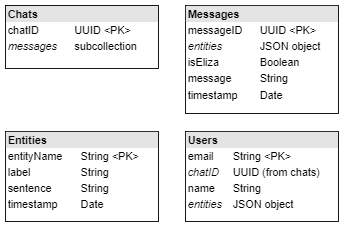
\includegraphics[width=\textwidth]{db-schema}
	\caption{Diagram showing the schema used for the database structure}
	\label{fig:db-schema}
\end{figure}
\section{System Overview}
Figure \ref{fig:system-diagram} shows an overview of the different components of the system and how they communicate and transfer data. The web application, which is going to be implemented in HTML, CSS and JavaScript, will communicate with the chatterbot, which will be implemented in Python, via web sockets. There are libraries, available both in Python and JavaScript which implement the same standard of web sockets making this functionality simple to implement and transfer small amounts of data. The web application will make use of Firebase Authentication, to securely authenticate users, and Firestore, as the database service. Both services will communicate to/from the web application using http calls via JavaScript libraries. Finally the web application will be hosted on a Flask server, which can be run on a localhost or can be deployed on a hosting platform, such as Heroku. One limitation of Heroku is that the free tier shuts down the server after 1 hour of inactivity and so there may be a short delay before the application becomes live again. \\
\begin{figure}[h]
	\centering
	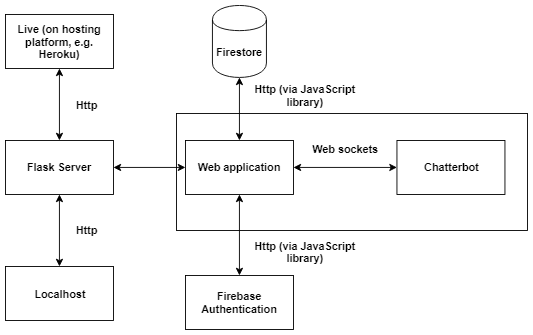
\includegraphics[width=\textwidth]{system-diagram}
	\caption{Diagram showing an overview of how the different components of the system are connected together}
	\label{fig:system-diagram}
\end{figure}
\section{Summary}
This chapter gave the reader a detailed look at the planning that was done prior to the implementation phase of this project. It first outlined the functional and non-functional requirements, including the level of priority. The functional requirements were written using the popular jobs to be done framework to show the different functional events and their expected outcomes. The design methodologies, programming languages, tools and services used to implement the product were then introduced and finally the database schema and system overview diagram were discussed. \\\\
The next chapter will discuss the work carried out during the implementation phase of this project.